\subsection{Emergency Path Planning}

\subsubsection{Objective and Cost Function}
\paragraph{Objective}
The key objective is to reduce the downtime and cost of operation of the drone. This means both the cost of damage to the drone through crashing and the difficulty of retrieval need consideration.
\paragraph{Cost Considerations}
For this specific usage case, path planning has to consider the probability of failure at all instances along the path. 
\paragraph{Cost Function}
Modelling the probability of surviving a node to node traversal between adjacent nodes as constant, $p$, the cost function of any path of length $D$ is shown in \ref{eq:cost function}.
\begin{equation}\label{eq:cost function}
    E(x) 
    = \sum_{n=1}^{D-1} c_{crashing}\bigl(x_n\bigr)\, (1-p) \,p^n 
    \;+\; c_{landing}\bigl(x_D\bigr)\, p^D
\end{equation}

\subsubsection{Weather induced failure}
\paragraph{Cause}
When a gust of wind exceeds the control capabilities of the drone it will cause an extreme disturbance and likely failure resulting in a crash. This is especially important to consider when their is an actuator fault due to the less aggressive control strategies deployed meaning that the maximum rejected gust becomes lower in magnitude and therefore more likely to occur. 
\paragraph{Gust Modelling}
Using the \textbf{Meteomatics API} forecast and modelling in \ref{SAM GRACE} the gustiness of the operating environment can be approximated. From this a model, the probability that a gust exceeds the known maximum rejection gust speed for the current control gains per second, $\lambda$, is calculated as shown in \ref{eq:p calc}. The specifics of the calculation of $\lambda$ are an area for future work, however, they would also greatly benefit from the collection of real-time data for the drone in testing.

\begin{equation}\label{eq:p calc}
    p = (1-\lambda)^{\frac{nodal\_distance}{speed}}
\end{equation}

\subsubsection{Search Algorithms}
\begin{algorithm}
\caption{Exhaustive Search}
\label{alg:search}
\begin{algorithmic}[1]
    \For{each Node $n$}
        \State $\textit{min\_cost} \gets \infty$
        \State $n.path\_cost$ = \Call{search}{$n$, $p$, $1$, $0$, $depth$, $\textit{min\_cost}$}
    \EndFor
    
    \Function{search}{$n$, $p$, $p\_alive$, $cost$, $depth$, \textbf{ref} $\textit{min\_cost}$}
        \State $\textit{current\_cost} \gets cost + p\_alive \cdot n.\textit{landing\_cost}$
        \If{$\textit{current\_cost} < \textit{min\_cost}$}
            \State $\textit{min\_cost} \gets \textit{current\_cost}$
        \EndIf
        \If{$depth = 0$ $\mathbf{or}$ $n.\textit{landing\_cost} = 0$ $\mathbf{or}$ $cost > \textit{min\_cost}$}
            \State \Return
        \EndIf
        \For{each $\textit{neighbour}$ in $n.\textit{neighbours}$}
            \State $p\_alive\_next \gets p\_alive \cdot p$
            \State $cost\_next \gets cost + p\_alive \cdot (1 - p) \cdot n.\textit{crashing\_cost}$
            \State \Call{search}{$\textit{neighbour}$, $p$, $p\_alive\_next$, $cost\_next$, $depth - 1$, $\textit{min\_cost}$}
        \EndFor
    \EndFunction
\end{algorithmic}
\end{algorithm}
\begin{algorithm}
    \caption{Smooth}
    \label{alg:flow}
\begin{algorithmic}[1]
    \While{not $Converged$}
        \State $Converged \gets TRUE$
        \For{each Node $n$}
            \For{each \textit{neighbour} in $n.\textit{neighbours}$}
                \State $\textit{movement\_cost} \gets n.\textit{crashing\_cost} \cdot \frac{1 - p}{2} +  \textit{neighbour}.\textit{crashing\_cost} \cdot \frac{p(1 - p)}{2}$
                \State $\textit{total\_cost} \gets \textit{movement\_cost} + p \cdot \textit{neighbour.path\_cost}$
                \If{$\textit{total\_cost} < n.\textit{path\_cost}$}
                    \State $n.\textit{path\_cost} \gets \textit{total\_cost}$
                    \State $Converged \gets FALSE$
                \EndIf
            \EndFor
        \EndFor
    \EndWhile
\end{algorithmic}
\end{algorithm}
\paragraph{Exhaustive Search}
The simplest and easiest to understand algorithm is a simple search algorithm as shown in \ref{alg:search}. This recursively calls search until it searches all viable lines. There are steps taken to increase the efficiency, including pruning lines that already exceed the minimum cost as the cost is monotonic increasing and automatically terminating lines when they are above the best terminal state possible. However, the worst case time complexity remains $O(|V|6^{depth})$ as each node has 6 neighbours that get called recursively, to get guaranteed correct results it would require searching all paths as long as $|V|$ as costs cannot fall below 0 so it is never advantageous to revisit a node. Therefore the worst case complexity for guaranteed optimal paths is $O(|V|6^{|V|})$ This is not usable for practical applications, therefore the user must compromise depth of search, no longer getting optimal path results.
\paragraph{Smoothing}
To combat the issues with \ref{alg:search}, \ref{alg:flow} was developed. The key idea behind this algorithm is that it smooths out the differences in path cost between neighbouring nodes. This means you get a guaranteed correct answers when the nodes have fully converged. This algorithm is a Bellman-Ford style algorithm and therefore has a time complexity of $O(|E|\times |V|)$ \cite{REF}. In dense graphs this becomes  $O(|V|^3)$ however, we know $|E| \leq |V| \times 7$ as we are using hexagons can have an edge to 6 neighbours and a self edge indicating landing, therefore the actual complexity is $O(|V|^2)$. 

\subsubsection{Real-time application}
\paragraph{Pre-Compute}
Carrying out memory and time complex operations on real-time hardware should always be avoided. This is because with real time systems, loops require specific timings for optimal use. Therefore, if we have algorithms that do not operate to precise timings the system can fail or be forced to be less efficient. If all the values are pre-computed and uploaded to the drone with the optimal path the time and memory complexity becomes $O(1)$ which supports precise, timed loops. Within the path planning workflow, as much as possible should be pre-computed and simply accessed, however, if any algorithms are deployed they should be $O(1)$ for predictable timing requirements.
\paragraph{$p$ ranges}
While the value of $p$ can take any value between 0 and 1, there can be only 7 outputs for the next best move (going to each of the 6 neighbours or landing). Therefore, instead of creating a specific map for a specific value of $p$ on the Flight Controller you can pre-compute all the ranges of $p$ that would cause each of these outcomes and get the exact same result for the only thing that matters to the drone, which action should be taken next.
\paragraph{Deployment}
For a deployed algorithm consistent timings and a minimal memory footprint are essential. This allows for the path planning loop to run at higher speeds as with lower memory requirements faster memory access forms are available and with consistent timings you can maintain consistency in looping speed. To reduce the memory intensity, instead of storing ranges of values you store a sorted array of values going from the smallest $p$ to the greatest. The first time the specific value of $p$ crosses the threshold $p$, you record the required action and if no value crosses the threshold then you default to landing. Finally, to convert row and column indexes instead of the nodes into \gls{GNSS} co-ordinates required for headings you can use a precomputed reference map to ensure reliable access times, or work it out using the scaling factor and a reference co-ordinate to reduce the memory requirements.
\paragraph{Memory Management}
The memory on the \gls{MCU}s consists of Flash and \gls{SRAM}. Flash is static memory that has to be pre-loaded onto the board before each run whereas \gls{SRAM} is volatile but has faster access times. Therefore, the optimal strategy is to load the waypoints, maps and gains from the preset values in Flash before a flight into \gls{SRAM}, these can be reload from Flash in cases of temporary power loss. Furthermore, the Flight Controllers \gls{MCU} contains 2 megabytes of Flash, 64 kilobytes of \gls{ITCM} configured \gls{RAM} 128 kilobytes of \gls{DTCM} configured \gls{RAM} \cite{REF}. These allow for precise timings and should therefore be used for looped processes including control loops and heading calculations. Whereas, for less timing critical actions or varying time operations such as actuator tests the regular \gls{SRAM} can be used. However, for the \gls{GNSS} module \gls{MCU} there is just 128 kilobytes of Flash and 32 kilobytes of \gls{SRAM}.
\paragraph{Memory Requirement Reduction}
Using the C implementation given in \ref{lst:easynode} it requires 56 bytes per node, therefore, for a 256 node map it requires 14.336 kilobytes of \gls{RAM}. While this is acceptable for the Flight Controller, it would be using over half of the available \gls{RAM} on the \gls{GNSS} Module. This puts significant resolution limitations on the map. Therefore, methods for memory reduction are important. To achieve this, the map should be stored in an array where the indexes where the specific attributes are reduced to the number of bits they reasonably require. 12 bits supports indexing up to 4096 nodes and 8 bits for probability values is more than sufficient. This leads to the 19 byte/node option in \ref{lst:node}, significantly reducing the memory intensity with no effect to performance. In addition, the nature of the problem can be exploited. In most cases, the map has one option for the next move that above a probability threshold it goes to, and below that threshold it lands. Therefore, you can store just the action and the probability threshold. Lastly, using a pair axial co-ordinates as outlined \cite{REF} you can encode the co-ordinates of the node in the index of the node, from these axial co-ordinates and the scaling factor the distance from the reference co-ordinate can be found. This leads to the \ref{lst:reducednode} reducing the memory per node to 2.5 bytes/node. Lastly, the precision of $p$ can be reduced and if the map is guaranteed to be below 256 nodes you can use the node shown in \ref{lst:ultrareducednode} that is just 1.5 bytes/node. 
\paragraph{Testing Reduced Nodes}
Using 10 random satellite images from the Kharkiv region, 256 node cost maps were generated including visible obstacles and assumed regions of interest. Then starting at each node of the region of interest 20 separate trials are run using the different nodal structures. Their performances are calculated using random failures in line with \textit{p}. The limitation of this method is the limited resolution and lack of actual real world data. To validate the models during the testing stage all cost maps should be recorded and used as as a testing set. The optimal results are calculated using \ref{lst:easynode}.

\paragraph{Reduced Nodes Performance Results}
The results in \ref{fig:Reduced Nodes} shows that the reduced mode performed equally to the optimal and the ultra reduced nodes only performed worse as $p$ approached 1. However, the reduced node methods can no longer guarantee optimal results leaving them vulnerable to unforeseen situations, furthermore the on-board computations required to mediate between the indexes and the locations increases the processing requirements. Therefore, the \ref{lst:node} should be implemented if possible before using the advanced options, as it guarantees optimal performance with 33.9\% the memory requirement as \ref{lst:easynode}.
\textbf{Can make a point about structuring so that the even with weird bit operations}

\begin{lstlisting}[caption={Implementated Node Structure},label={lst:easynode}]
struct Node {
    float rel_long, rel_lat;  // relative longitude and lattidue to reference point
    float p_values[6];        // Probability thresholds
    Node* actions[6];         // Points to the next node
};
\end{lstlisting}
% total bits/node = 448 / 56 bytes
\begin{lstlisting}[caption={Node Structure},label={lst:node}]
struct Node {
    rel_long, rel_lat;  // relative longitude and lattidue to reference point, 16 bit numbers
    p_values[6];    // Probability thresholds, 8 bit numbers
    actions[6];     // Indexes of the next node, 12 bit numbers
};
\end{lstlisting}
% total bits/node = 120 bits / 15 bytes
\begin{lstlisting}[caption={Reduced Node Structure},label={lst:reducednode}]
struct ReducedNode {
    p_thresh;                // Probability threshold, 8 bit number
    action;                  // Connected node, 12 bit number
};
\end{lstlisting}
% total bits/node = 20 bits /  2.5 bytes
\begin{lstlisting}[caption={Ultra Reduced Node Structure},label={lst:ultrareducednode}]
struct UltraReducedNode {
    p_thresh;                // Probability threshold, 4 bit number
    action;                  // Connected node, 8 bit number
};
\end{lstlisting}
%total bits/node = 12 bits / 1.5 bytes
\begin{figure}[htbp]
  \centering
  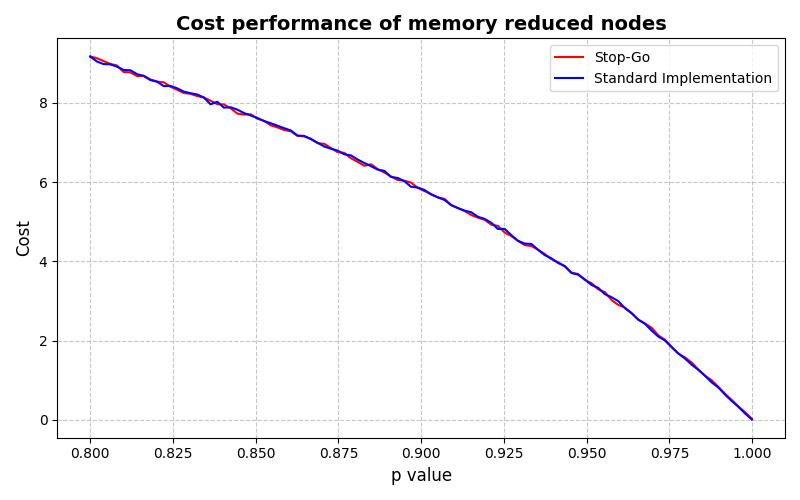
\includegraphics[width=1\textwidth]{figs/Thomas/Return To Safety/Reduced Nodes.png}
  \caption[Memory Reduced Nodes Performance]{Simulated results using Kharkiv test data based on method described in \ref{sub_sub_section:tgt_testing_sims} and the cost function in \ref{sub_sub_section:tgt_cost_function}}
  \label{fig:Reduced Nodes}
\end{figure}
